\documentclass[11pt,a4paper]{article}
\usepackage[utf8]{inputenc}
\usepackage[margin=1in]{geometry}
\usepackage{amsmath, amssymb, amsfonts}
\usepackage{booktabs}
\usepackage{hyperref}
\usepackage{tikz}
\usetikzlibrary{shapes.geometric, arrows, positioning}

\title{\textbf{Algorithm Specification: Spatial Rolling WS-LR QAOA with Receding-Horizon Batch Commitment \& LNS (Hybrid 2+5)}}
\author{Technical Documentation}
\date{\today}

\begin{document}

\maketitle

\section{High-Level System Architecture}

The \textbf{Spatial Rolling Warm-Start Linear Relaxation Quantum Alternating Operator Algorithm with Receding-Horizon Batch Commitment and Large Neighborhood Search (Hybrid 2+5)} is a domain-decomposed quantum-classical hybrid solver designed for the \textbf{Open Traveling Salesperson Problem (Open TSP)}.

Directly mapping an $n$-city TSP onto a quantum computer using positional binary encoding requires $n^2$ qubits, which quickly exceeds the fidelity limits and qubit capacities of modern Near-Term Intermediate-Scale Quantum (NISQ) devices. The Hybrid 2+5 architecture resolves this scalability barrier by decomposing the global Open TSP into a sequence of small, localized sub-problems solved iteratively on a rolling spatial window.

\begin{figure}[h!]
\centering
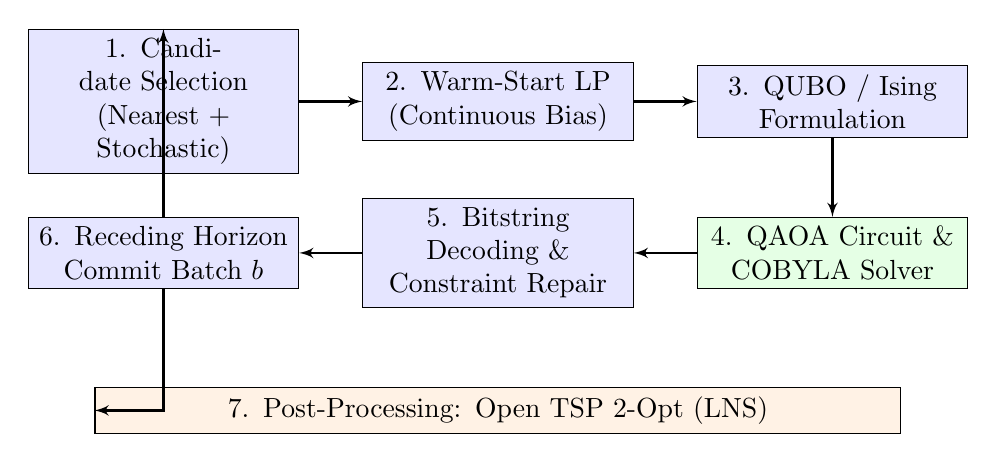
\begin{tikzpicture}[node distance=1.5cm, auto, >=latex', every node/.style={transform shape}]
    \node [draw, rectangle, fill=blue!10, text width=3.2cm, align=center] (cand) {1. Candidate Selection\\(Nearest + Stochastic)};
    \node [draw, rectangle, fill=blue!10, text width=3.2cm, align=center, right=0.8cm of cand] (lp) {2. Warm-Start LP\\(Continuous Bias)};
    \node [draw, rectangle, fill=blue!10, text width=3.2cm, align=center, right=0.8cm of lp] (qubo) {3. QUBO / Ising\\Formulation};
    \node [draw, rectangle, fill=green!10, text width=3.2cm, align=center, below=1.0cm of qubo] (qaoa) {4. QAOA Circuit \&\\COBYLA Solver};
    \node [draw, rectangle, fill=blue!10, text width=3.2cm, align=center, left=0.8cm of qaoa] (decode) {5. Bitstring Decoding \&\\Constraint Repair};
    \node [draw, rectangle, fill=blue!10, text width=3.2cm, align=center, left=0.8cm of decode] (commit) {6. Receding Horizon\\Commit Batch $b$};
    \node [draw, rectangle, fill=orange!10, text width=10cm, align=center, below=1.0cm of decode] (lns) {7. Post-Processing: Open TSP 2-Opt (LNS)};

    \draw[->, thick] (cand) -- (lp);
    \draw[->, thick] (lp) -- (qubo);
    \draw[->, thick] (qubo) -- (qaoa);
    \draw[->, thick] (qaoa) -- (decode);
    \draw[->, thick] (decode) -- (commit);
    \draw[->, thick] (commit.north) -- ++(0,0.5) -| (cand.north);
    \draw[->, thick] (commit) |- (lns);
\end{tikzpicture}
\caption{Global Rolling Subtour System Execution Lifecycle.}
\end{figure}

---

\section{Problem Formulation: Open Traveling Salesperson Problem}

Let $G = (V, E)$ be a complete graph where $V = \{0, 1, \dots, n-1\}$ represents the set of $n$ nodes, and $E = V \times V$ represents the directed edges with associated distance/cost matrix $M \in \mathbb{R}_{\ge 0}^{n \times n}$. 

Unlike the classic Closed TSP, the \textbf{Open TSP} seeks a Hamiltonian path $T = (v_0, v_1, \dots, v_{n-1})$ starting at a fixed depot node $v_0 = v_{\text{depot}}$ that visits every node in $V$ exactly once, without returning to $v_0$ at the end. The objective is to minimize the total path distance:
\begin{equation}
\mathcal{C}(T) = \sum_{m=0}^{n-2} M_{v_m, v_{m+1}}
\end{equation}

---

\section{Spatial Candidate Selection \& Stochastic Exploration}

At any step along the path creation process, let $v_{\text{curr}}$ be the most recently committed node, and let $U \subset V$ be the set of unvisited nodes ($|U| \le n$). 

To constrain the quantum sub-problem to a fixed maximum qubit allocation $K = \text{qubit\_count}$, the algorithm dynamically samples a candidate subset $S \subseteq U$ of size $k = \min(K, |U|)$. The selection balances deterministic local greedy choices with stochastic exploration governed by an exploration fraction $\eta \in [0, 1]$:

\begin{enumerate}
    \item \textbf{Exploration Budget Allocation:}
    \begin{equation}
    n_{\text{explore}} = \begin{cases} 0 & \text{if } \eta = 0 \\ \min\left(\lfloor k \cdot \eta \rfloor, k - 1\right) & \text{if } \eta > 0 \text{ and } k > 1 \end{cases}
    \end{equation}
    \begin{equation}
    n_{\text{nearest}} = k - n_{\text{explore}}
    \end{equation}

    \item \textbf{Nearest-Neighbor Candidate Set ($S_{\text{near}}$):}
    Unvisited nodes in $U$ are sorted in ascending order according to distance from the current node $v_{\text{curr}}$, using node index $x$ as a deterministic tie-breaker:
    \begin{equation}
    \text{Key}(x) = \left(M_{v_{\text{curr}}, x}, x\right)
    \end{equation}
    The first $n_{\text{nearest}}$ elements of this sorted list form $S_{\text{near}}$.

    \item \textbf{Stochastic Exploration Candidate Set ($S_{\text{explore}}$):}
    If $n_{\text{explore}} > 0$, $n_{\text{explore}}$ candidates are uniformly sampled at random without replacement from the remaining unvisited set $U \setminus S_{\text{near}}$.

    \item \textbf{Combined Subtour Candidates:}
    \begin{equation}
    S = S_{\text{near}} \cup S_{\text{explore}} = \{c_0, c_1, \dots, c_{k-1}\}
    \end{equation}
\end{enumerate}

---

\section{Continuous Linear Relaxation Warm-Start (WS-LR)}

Standard QAOA initializes all qubits in an equal superposition state $|+\rangle^{\otimes N}$. To accelerate convergence and guide the quantum state toward low-energy subspace regions, the algorithm solves a continuous \textbf{Linear Programming (LP) Relaxation} over the candidate subtour $S$.

\subsection{LP Continuous Formulation}
We define continuous decision variables $x_{i,t} \in [0, 1]$ representing the relaxed probability that candidate $c_i \in S$ is assigned to step $t \in \{0, 1, \dots, k-1\}$ of the localized subtour.

\begin{equation}
\min_{\mathbf{x}} \quad \sum_{i=0}^{k-1} M_{v_{\text{curr}}, c_i} x_{i,0} + \sum_{t=0}^{k-2} \sum_{i=0}^{k-1} \left( \frac{1}{2} \sum_{j \neq i}^{k-1} M_{c_i, c_j} \right) x_{i,t}
\end{equation}

Subject to the assignment constraints:
\begin{align}
\sum_{t=0}^{k-1} x_{i,t} &= 1 \quad \forall i \in \{0, \dots, k-1\} \quad \text{(Each candidate visited once)} \\
\sum_{i=0}^{k-1} x_{i,t} &= 1 \quad \forall t \in \{0, \dots, k-1\} \quad \text{(Each position occupied once)} \\
0 \le x_{i,t} &\le 1 \quad \forall i, t \in \{0, \dots, k-1\}
\end{align}

If the linear program fails to converge, a uniform distribution $x_{i,t} = \frac{1}{k}$ is assigned.

\subsection{Initial Angle Generation}
The resulting optimal continuous solution $\mathbf{x}^{\text{LP}}$ is clipped to a numerically stable range $[\epsilon, 1-\epsilon]$ with $\epsilon = 10^{-4}$, and mapped to initial single-qubit Bloch sphere rotation angles $\theta_{\alpha}$:
\begin{equation}
\theta_{\alpha} = 2 \arcsin\left(\sqrt{x^{\text{LP}}_{\alpha}}\right), \quad \text{where } \alpha = i \cdot k + t
\end{equation}

---

\section{QUBO Formulation \& Ising Mapping}

To optimize the candidate sequence on quantum hardware, the localized Open TSP is mapped onto a Quadratic Unconstrained Binary Optimization (QUBO) problem over $N = k^2$ binary variables:
\begin{equation}
x_{\alpha} = x_{i,t} \in \{0, 1\}, \quad \text{indexed by } \alpha(i,t) = i \cdot k + t
\end{equation}

\subsection{QUBO Energy Objective Function}
The objective function balances path costs with quadratic penalty terms enforced by multiplier $P = 100.0$:
\begin{equation}
E(\mathbf{x}) = \mathbf{x}^T Q \mathbf{x} = H_{\text{cost}}(\mathbf{x}) + P \cdot H_{\text{penalty}}(\mathbf{x})
\end{equation}

\begin{enumerate}
    \item \textbf{Path Cost Terms:}
    \begin{equation}
    H_{\text{cost}}(\mathbf{x}) = \sum_{i=0}^{k-1} M_{v_{\text{curr}}, c_i} x_{i,0} + \sum_{t=0}^{k-2} \sum_{i=0}^{k-1} \sum_{j \neq i}^{k-1} M_{c_i, c_j} x_{i,t} x_{j,t+1}
    \end{equation}

    \item \textbf{Assignment Penalty Terms:}
    \begin{equation}
    H_{\text{penalty}}(\mathbf{x}) = \sum_{i=0}^{k-1} \left( \sum_{t=0}^{k-1} x_{i,t} - 1 \right)^2 + \sum_{t=0}^{k-1} \left( \sum_{i=0}^{k-1} x_{i,t} - 1 \right)^2
    \end{equation}
\end{enumerate}

\subsection{Explicit QUBO Matrix Entries}
Using the expansion $(y - 1)^2 = y^2 - 2y + 1$, and recognizing that $x^2 = x$ for $x \in \{0, 1\}$, the non-zero coefficients of matrix $Q \in \mathbb{R}^{k^2 \times k^2}$ are defined as:

\begin{itemize}
    \item \textbf{Diagonal Terms:}
    \begin{equation}
    Q_{(i,t), (i,t)} = \begin{cases} M_{v_{\text{curr}}, c_i} - 2P & \text{if } t = 0 \\ -2P & \text{if } t > 0 \end{cases}
    \end{equation}

    \item \textbf{Off-Diagonal Penalty Constraints:}
    \begin{align}
    Q_{(i,t_1), (i,t_2)} &= P \quad \forall t_1 \neq t_2 \quad \text{(Row uniqueness constraints)} \\
    Q_{(i_1,t), (i_2,t)} &= P \quad \forall i_1 \neq i_2 \quad \text{(Column uniqueness constraints)}
    \end{align}

    \item \textbf{Off-Diagonal Edge Cost Transitions:}
    \begin{equation}
    Q_{(i,t), (j,t+1)} = M_{c_i, c_j} \quad \forall i \neq j, \forall t \in \{0, \dots, k-2\}
    \end{equation}
\end{itemize}

\subsection{Ising Transformation}
The binary variables $x_\alpha$ are converted to Pauli-$Z$ spin operators via the canonical substitution $x_\alpha \mapsto \frac{I - Z_\alpha}{2}$, producing the problem Cost Hamiltonian:
\begin{equation}
H_C = \sum_{\alpha=0}^{N-1} Q_{\alpha,\alpha} \left(\frac{I - Z_\alpha}{2}\right) + \sum_{\alpha < \beta} \left(Q_{\alpha,\beta} + Q_{\beta,\alpha}\right) \left(\frac{I - Z_\alpha}{2}\right)\left(\frac{I - Z_\beta}{2}\right)
\end{equation}

---

\section{Quantum Circuit Construction \& Variational QAOA}

The algorithm synthesizes a parameterized quantum circuit of depth $p$ ($p$-layers) acting on $N = k^2$ qubits.

\subsection{1. State Preparation Layer}
Instead of standard Hadamard initialization, qubits are biased using the continuous LP angles $\theta_\alpha$:
\begin{equation}
|\psi_0\rangle = \bigotimes_{\alpha=0}^{N-1} R_Y(\theta_\alpha)|0\rangle = \bigotimes_{\alpha=0}^{N-1} \left( \cos\frac{\theta_\alpha}{2}|0\rangle + \sin\frac{\theta_\alpha}{2}|1\rangle \right)
\end{equation}

\subsection{2. Cost Phase Separator Unitary $U(H_C, \gamma)$}
For layer $l \in \{1, \dots, p\}$ with variational parameter $\gamma_l$:
\begin{equation}
U(H_C, \gamma_l) = e^{-i \gamma_l H_C} = \prod_{\alpha=0}^{N-1} R_Z\left(2 \gamma_l Q_{\alpha,\alpha}\right) \prod_{\alpha < \beta} R_{ZZ}\left(\gamma_l (Q_{\alpha,\beta} + Q_{\beta,\alpha})\right)
\end{equation}
where $R_{ZZ}(\theta) = e^{-i \frac{\theta}{2} (Z \otimes Z)}$.

\subsection{3. Mixer Layer $U(H_M, \beta_l)$}
Depending on the configuration flag \texttt{xy\_mixer}, one of two mixer architectures is chosen:

\begin{itemize}
    \item \textbf{Warm-Start Custom X-Mixer (WS-X):}
    Applies non-axis-aligned rotations that preserve invariant properties around initial state angles $\theta_\alpha$:
    \begin{equation}
    U(H_M, \beta_l) = \prod_{\alpha=0}^{N-1} R_Y(-\theta_\alpha) \, R_X(2 \beta_l) \, R_Y(\theta_\alpha)
    \end{equation}

    \item \textbf{XY Ring Mixer:}
    Applies particle-number-preserving entangling gates across adjacent qubits:
    \begin{equation}
    U_{\text{XY}}(\beta_l) = \prod_{\alpha=0}^{N-2} R_{XX}(\beta_l) \, R_{YY}(\beta_l)
    \end{equation}
\end{itemize}

\subsection{4. Classical Parameter Optimization}
The circuit expectation value is minimized over continuous parameters $\boldsymbol{\gamma}, \boldsymbol{\beta} \in \mathbb{R}^p$:
\begin{equation}
\min_{\boldsymbol{\gamma}, \boldsymbol{\beta}} \langle \psi(\boldsymbol{\gamma}, \boldsymbol{\beta}) | H_C | \psi(\boldsymbol{\gamma}, \boldsymbol{\beta}) \rangle
\end{equation}
The optimization is performed classically using the \textbf{COBYLA} algorithm over a maximum of 30 function evaluations.

---

\section{Bitstring Decoding \& Constraint Repair}

Sampling the optimized statevector produces a probability distribution over bitstrings $\mathbf{b} \in \{0, 1\}^{k^2}$. The bitstring yielding the lowest classical energy $E(\mathbf{b}) = \mathbf{b}^T Q \mathbf{b}$ is extracted and parsed into a $k \times k$ assignment grid $B_{i,t} = b_{i \cdot k + t}$.

Because quantum sampling may yield infeasible states violating 1-hot constraints, a deterministic \textbf{Greedy Constraint Repair Scheme} decodes $B$ into a valid candidate permutation tour:

\begin{enumerate}
    \item Maintain an empty ordered subtour list $L$ and a set of assigned candidates $V_{\text{assigned}} = \emptyset$.
    \item For each time step $t = 0, 1, \dots, k-1$:
    \begin{itemize}
        \item Select candidate $i^* = \arg\max_{i \notin V_{\text{assigned}}} B_{i,t}$.
        \item If all remaining candidates have equal value, pick the candidate with the lowest index $i$.
        \item Append candidate $c_{i^*}$ to $L$ and add $i^*$ to $V_{\text{assigned}}$.
    \end{itemize}
    \item Output repaired subtour sequence $L = (c_{\pi(0)}, c_{\pi(1)}, \dots, c_{\pi(k-1)})$.
\end{enumerate}

---

\section{Receding-Horizon Batch Commitment}

To prevent cumulative decision errors and sub-optimal local traps, the algorithm uses a \textbf{Receding-Horizon Policy}:

\begin{enumerate}
    \item Out of $k$ nodes present in the evaluated subtour $L$, only the first $b = \min(\text{batch\_count}, k)$ nodes are committed to the global path $T$:
    \begin{equation}
    \text{Commit Set} = \{ L[0], L[1], \dots, L[b-1] \}
    \end{equation}
    \item The global path is updated: $T \leftarrow T \mathbin{\Vert} \text{Commit Set}$.
    \item These $b$ nodes are permanently removed from the unvisited set $U$:
    \begin{equation}
    U \leftarrow U \setminus \text{Commit Set}
    \end{equation}
    \item The current active node is updated to the last committed node:
    \begin{equation}
    v_{\text{curr}} \leftarrow L[b-1]
    \end{equation}
    \item The spatial window rolls forward, and candidate selection repeats until $U = \emptyset$.
\end{enumerate}

---

\section{Large Neighborhood Search (Open TSP 2-Opt)}

Once all $n$ nodes have been incorporated into global path $T = (v_0, v_1, \dots, v_{n-1})$, a classical \textbf{2-Opt Local Neighborhood Search (LNS)} post-processing pass refines the tour sequence.

\subsection{Open TSP Edge Exchange Evaluation}
For indices $1 \le i < j \le n - 1$, swapping intermediate path segment $T[i : j+1]$ alters total path cost by $\Delta \mathcal{C} = \mathcal{C}_{\text{new}} - \mathcal{C}_{\text{old}}$:

\begin{itemize}
    \item \textbf{Case 1: Intermediate Swaps ($j < n - 1$)}
    \begin{equation}
    \Delta \mathcal{C} = \left( M_{v_{i-1}, v_j} + M_{v_i, v_{j+1}} \right) - \left( M_{v_{i-1}, v_i} + M_{v_j, v_{j+1}} \right)
    \end{equation}

    \item \textbf{Case 2: Terminal Swaps ($j = n - 1$)}
    \begin{equation}
    \Delta \mathcal{C} = M_{v_{i-1}, v_j} - M_{v_{i-1}, v_i}
    \end{equation}
\end{itemize}

If $\Delta \mathcal{C} < 0$, the sub-segment $T[i : j+1]$ is reversed in-place:
\begin{equation}
T_{\text{updated}} = (v_0, \dots, v_{i-1}, \mathbf{v_j, v_{j-1}, \dots, v_i}, v_{j+1}, \dots, v_{n-1})
\end{equation}

---

\section{Summary of Algorithm Parameters}

\begin{table}[h!]
\centering
\begin{tabular}{@{}llll@{}}
\toprule
\textbf{Parameter} & \textbf{Symbol} & \textbf{Range / Type} & \textbf{Description} \\ \midrule
\texttt{qubit\_count} & $K$ & $\mathbb{Z}_{\ge 1}$ & Maximum size of local candidate subtour $k = \min(K, |U|)$. \\
\texttt{exploration\_percent} & $\eta$ & $[0.0, 1.0]$ & Ratio of stochastic unvisited candidates vs. nearest neighbors. \\
\texttt{batch\_count} & $b$ & $[1, K]$ & Number of subtour nodes committed per rolling window iteration. \\
\texttt{xy\_mixer} & - & \texttt{Boolean} & Toggles Warm-Start X-Mixer vs. XY Ring Entangling Mixer. \\
\texttt{p\_layers} & $p$ & $\mathbb{Z}_{\ge 1}$ & Number of alternating cost/mixer layers in the QAOA circuit. \\
\texttt{penalty} & $P$ & $\mathbb{R}_{> 0}$ & Penalty multiplier for 1-hot positional encoding constraints. \\ \bottomrule
\end{tabular}
\caption{Configuration parameters controlling the Hybrid 2+5 algorithm execution.}
\end{table}

\end{document}